\chapter{Manual de Usuario} \label{cap:manual_usuario}

En este capítulo se proporciona un manual de usuario para la aplicación desarrollada, se explicará cómo ejecutar el pipeline completo de manera sencilla. Para obtener más información técnica sobre la implementación, se recomienda revisar los capítulos anteriores.

Para ejecutar la aplicación, simplemente hay que clickar en el archivo ejecutable \texttt{droplet\_analyzer.exe}.

\section{Interfaz Gráfica: Visión General}

Como se vió en el apartado 4.2.2 Descripción de la interfaz \ref{subsec:descripcion_interfaz}, la ventana principal se divide en seis secciones principales:
\begin{itemize}
    \item Sección 1 - Cargar Video: selección del fichero de vídeo de entrada.
    \item Sección 2 - Calibración: conversión de píxeles a unidades reales y ajuste de FPS.
    \item Sección 3 - Nombres de Salida: personalización de los nombres de los archivos generados.
    \item Sección 4 - Parámetros de Procesamiento: ajuste de todos los umbrales y filtros del algoritmo.
    \item Sección 5 - Procesamiento: botones de acción, barra de progreso.
    \item Sección 6 - Log de procesamiento y estadísticas.
\end{itemize}
    
\begin{figure}[H]
    \centering
    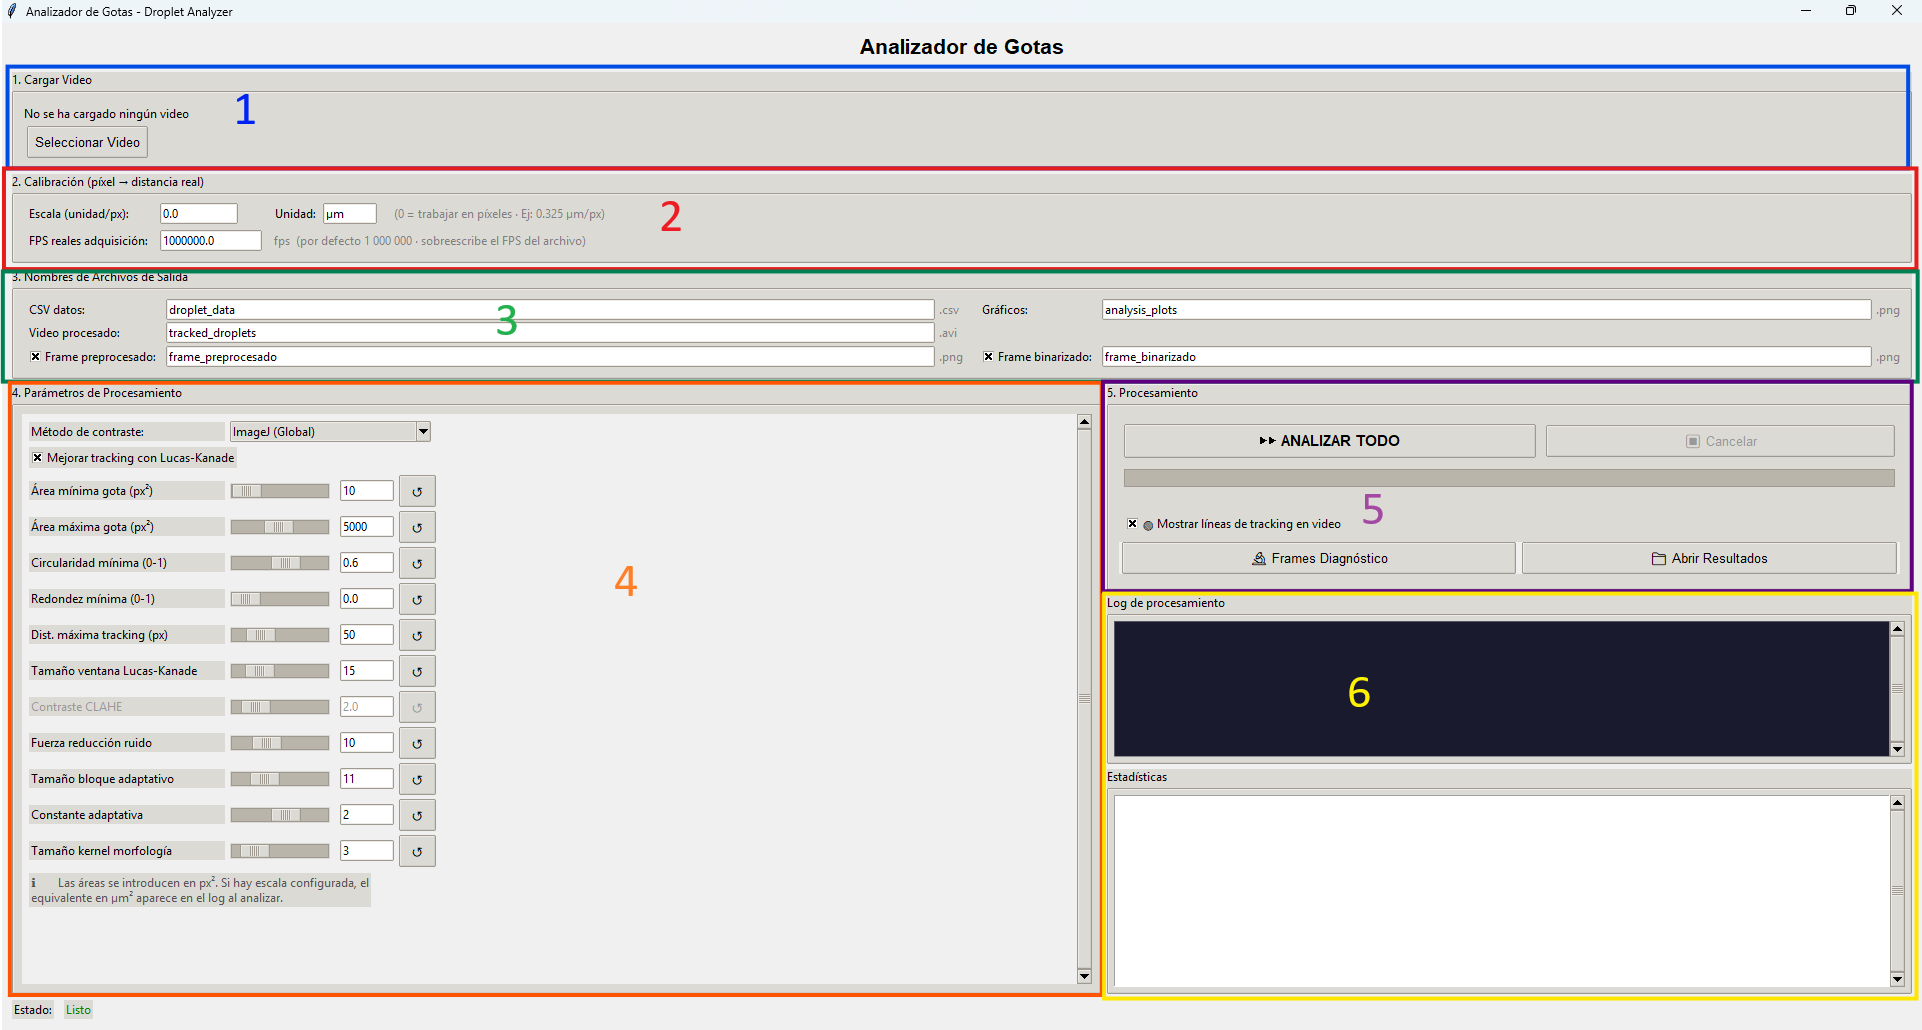
\includegraphics[width=0.9\textwidth]{figures/manual_usuario/desc_interfaz.png}
    \caption{Interfaz gráfica de la aplicación.}
\end{figure}

\section{Procedimiento}

Para analizar un vídeo, el usuario debe seguir los pasos que se detallan en esta sección.

\subsection{Paso 1: Cargar el vídeo}

La carga del vídeo se realiza siguiendo los siguientes pasos en el panel 1:
\begin{enumerate}
    \item Pulsar en el botón \textbf{Seleccionar Vídeo} para abrir el explorador de archivos \ref{fig:cargar_video_a}.
    \item Navegar hasta la ubicación del vídeo a analizar y seleccionarlo \ref{fig:cargar_video_b}.
    \item Una vez cargado, aparecerá el nombre del archivo, los fps y el número de fotogramas \ref{fig:cargar_video_c}.
\end{enumerate}

\begin{figure}[H]
    \centering
    
    \begin{subfigure}[b]{0.5\textwidth}
        \centering
        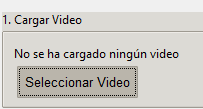
\includegraphics[width=\textwidth]{figures/manual_usuario/CargarVideo1.png}
        \caption{Botón para cargar el vídeo.}
        \label{fig:cargar_video_a}
    \end{subfigure}
    
    \vspace{0.5cm}
    
    \begin{subfigure}[b]{0.6\textwidth}
        \centering
        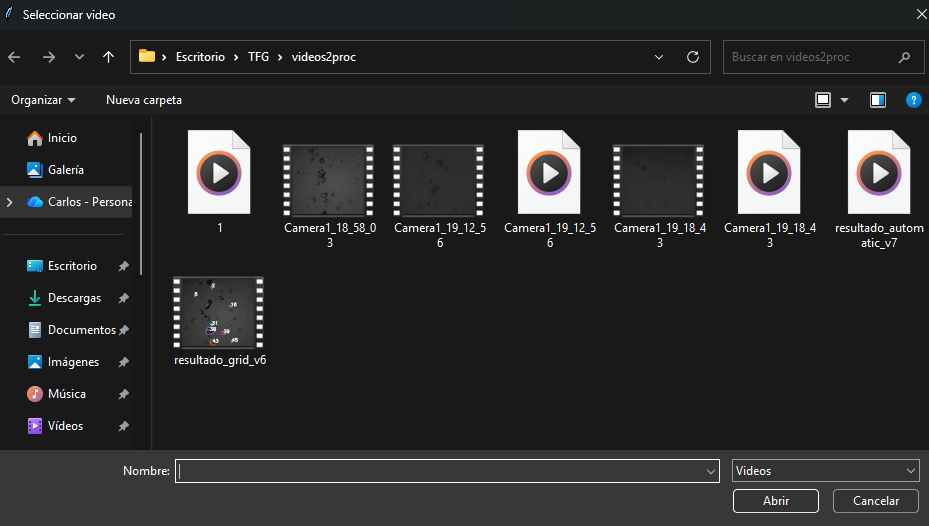
\includegraphics[width=\textwidth]{figures/manual_usuario/CargarVideo2.png}
        \caption{Seleccionar video.}
        \label{fig:cargar_video_b}
    \end{subfigure}

    \vspace{0.5cm}

    \begin{subfigure}[b]{0.5\textwidth}
        \centering
        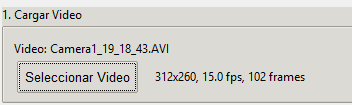
\includegraphics[width=\textwidth]{figures/manual_usuario/CargarVideo3.png}
        \caption{Vídeo cargado.}
        \label{fig:cargar_video_c}
    \end{subfigure}

    \caption{Proceso de carga del vídeo.}
    \label{fig:grupo_total}
\end{figure}

\subsection{Paso 2: Calibración (Escala y FPS)}

Una vez cargado el vídeo, hay que convertir los píxeles a unidades reales y ajustar la tasa de fotogramas reales. Para ello, se deben seguir los siguientes pasos en el panel 2:

\begin{enumerate}
    \item Introducir el factor de conversión de píxeles a unidades reales en el campo \textbf{Escala (unidad/px)}. Si el campo se deja a 0, todos los cálculos se realizarán en píxeles.
    \item Introducir los FPS reales a los que se grabó el vídeo en el campo de entrada \textbf{FPS reales adquisición}. Por defecto toma un valor de $10^{6}$ FPS.
\end{enumerate}

\begin{figure}[H]
    \centering
    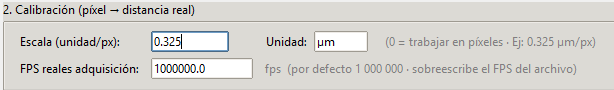
\includegraphics[width=0.8\textwidth]{figures/manual_usuario/Calibracion.png}
    \caption{Panel de calibración.}
\end{figure}

Cabe destacar que el factor de conversión depende del objetivo(zoom) con el que se haya grabado el vídeo, por lo que deberá recalibrarse para cada combinación de zoom y distancia al inyector utilizada en el experimento.

\textbf{Nota:} El campo \textbf{Unidad} es puramente descriptivo y no implica ninguna conversión automática. El usuario debe asegurarse de que el factor numérico introducido sea coherente con la unidad indicada y con el zoom utilizado durante la grabación.

\subsection{Paso 3: Nombres de archivos de salida}

En esta sección (Panel 3) se personalizan los nombres base de todos los ficheros que la
aplicación generará en la carpeta \texttt{output/}. Las extensiones se añaden
automáticamente. Nombres a configurar:
\begin{itemize}
    \item \textbf{Nombre base de CSV datos}: nombre del fichero principal de datos (defecto: droplet\_data.csv).
    \item \textbf{Nombre base de gráficos estadísticos}: nombre del fichero de gráficos estadísticos en PNG (defecto:analysis\_plots.png).
    \item \textbf{Nombre base de vídeo de salida}: nombre del vídeo que se genera con la visualización del procesamiento (defecto: tracked\_droplets.avi).
    \item \textbf{Frame preprocesado}: PNG del primer fotograma tras el preprocesado (activo con el checkbox).
    \item \textbf{Frame binarizado}: PNG del primer fotograma binarizado/segmentado (activo con el checkbox).
\end{itemize}

\begin{figure}[H]
    \centering
    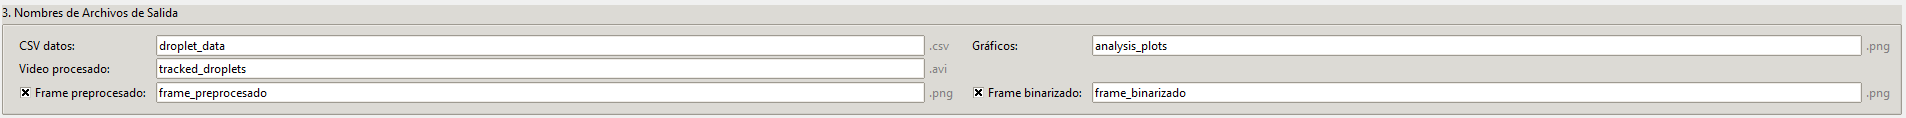
\includegraphics[width=1\textwidth]{figures/manual_usuario/nombres.png}
    \caption{Panel de configuración de nombres de salida.}
\end{figure}

\subsection{Paso 4: Parámetros de procesamiento}
En el panel 4 se configuran todos los parámetros relacionados con el procesamiento de vídeo. Dispone de un selector para elegir entre diferentes procesamientos del histograma, un checbox para activar o desactivar Lucas-Kanade, y varios campos de entrada con sliders para configurar los parámetros numéricos. Para más detalles de los parámetros, consultar la tabla \ref{tab:parametros_gui}.

En la figura \ref{fig:parametros} se muestra el panel de configuración de parámetros. El recuadro A corresponde al botón de reseteo al valor por defecto, el recuadro B al campo de entrada numérico y el recuadro C al slider.

\begin{figure}[H]
    \centering
    \includegraphics[width=0.85\textwidth]{figures/manual_usuario/parametros.png}
    \caption{Panel de configuración de parámetros de procesamiento.}
    \label{fig:parametros}
\end{figure}

\subsection{Paso 5: Procesamiento}

La ejecución del procesamiento se controla desde el panel 5. Para iniciar el procesamiento hay que pulsar el botón \textbf{Analizar Todo}. Esto analizará el vídeo completo, generando todos lo archivos de salida en la carpeta \texttt{output/}.
Antes de lanzar el procesamiento, podemos desactivar el checkbox \textbf{Mostrar líneas de tracking de vídeo} para que en el vídeo de salida no se pinten las trazas del seguimiento de las gotas.
Durante el procesamiento, la barra de progreso se va actualizando para mostrar el avance. El log de procesamiento (Panel 6) nos mostrará en tiempo real logs del procesamiento.

Si pulsamos el botón \texttt{Cancelar} se detendrá el análisis en el siguiente fotograma sin generar los archivos de salida.

\begin{figure}[H]
    \centering
    \includegraphics[width=0.9\textwidth]{figures/manual_usuario/procesamiento1.png}
    \caption{Panel de control de procesamiento.}
    \label{fig:procesamiento}
\end{figure}

Durante el procesamiento se abre una ventana flotante para previsualizar el análisis en tiempo real. Se muestra el fotograma original, el preprocesado, el binrizado y el final con las gotas detectadas y las líneas de tracking (si el checkbox está activo).

\begin{figure}[H]
    \centering
    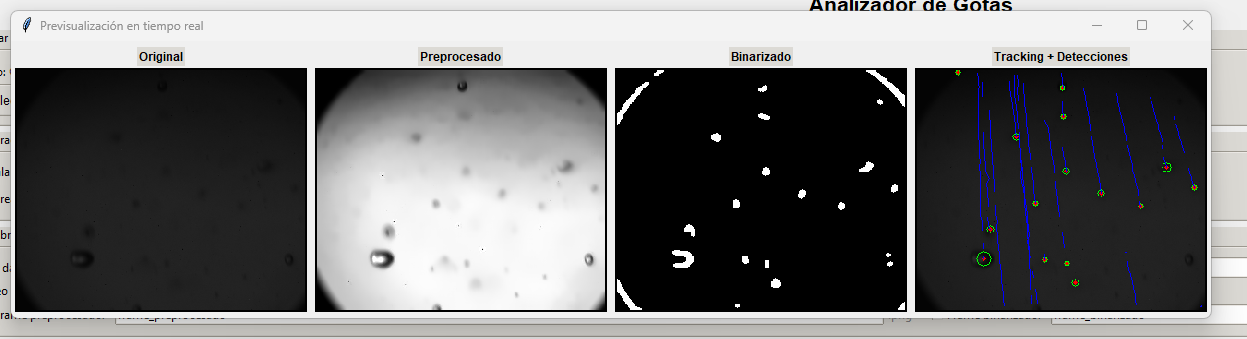
\includegraphics[width=0.9\textwidth]{figures/manual_usuario/previsualizacion.png}
    \caption{Ventana de previsualización en tiempo real.}
    \label{fig:previsualizacion}
\end{figure}

Una vez finalizado el procesamiento, aparecerán las estadísticas generales en la sección de log (Panel 6). Si pulsamos el botón \textbf{Abrir resultados} se abrirá la carpeta \texttt{output/} en el explorador de archivos.

\begin{figure}[H]
    \centering
    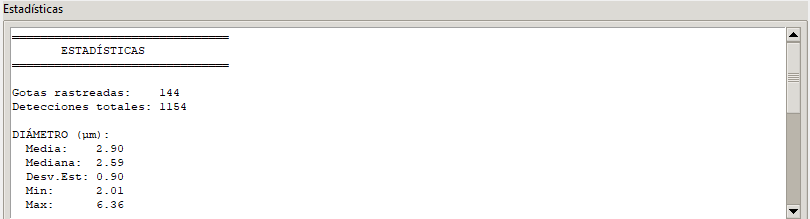
\includegraphics[width=0.9\textwidth]{figures/manual_usuario/estadisticas.png}
    \caption{Sección de estadísticas.}
    \label{fig:estadisticas}
\end{figure}

\section{Flujo recomendado para el ajuste de parámetros}

Para ajustar los parámetros de manera eficiente, sin lanzar el análisis completo cada vez, se recomienda seguir el siguiente flujo de trabajo:
\begin{enumerate}
    \shorthandoff{"}
    \item Cargue el vídeo y haga clic en "Frames Diagnóstico" sin cambiar ningún parámetro.
    \item Observe el frame binarizado. Si hay demasiado ruido, aumente  "Fuerza reducción" ruido o "Tamaño kernel morfología".
    \item Si las gotas no se detectan (aparecen en negro), ajuste "Constante adaptativa" o "Tamaño bloque adaptativo".
    \item Filtre por tamaño usando "Área mínima" y "Área máxima" para excluir artefactos.
    \item Ajuste "Circularidad mínima" o "Redondez mínima" según la forma real de sus gotas.
    \item Una vez satisfecho con la segmentación, lance el análisis completo.
\end{enumerate}

\section{Archivos de salida}

Al terminar el análisis se generan en la carpeta \texttt{output/} los siguientes archivos con información útil:

\begin{itemize}
    \item \textbf{CSV general}: Contiene información de las diferentes medidas por frame y track\_id.
    \item \textbf{Video de salida}: Contiene el vídeo procesado con las gotas detectadas y las líneas de tracking.
    \item \textbf{CSVs individuales}: Varios archivos CSV con la información de los ejes de las gráficas generadas.
    \item \textbf{Gráficas}: Archivos de imagen con las gráficas generadas a partir de los datos procesados.
    \item \textbf{Frames de diagnóstico}: Imagenes PNG del primer frame tras aplicar el preprocesado y la binarización.
\end{itemize}

En la figura \ref{fig:graficas} se muestra un ejemplo de las gráficas generadas a partir de los datos procesados. Estas gráficas incluyen información sobre la distribución de tamaños de gotas, velocidades, trayectorias, entre otras métricas relevantes para el análisis de las gotas.

\begin{figure}[H]
    \centering
    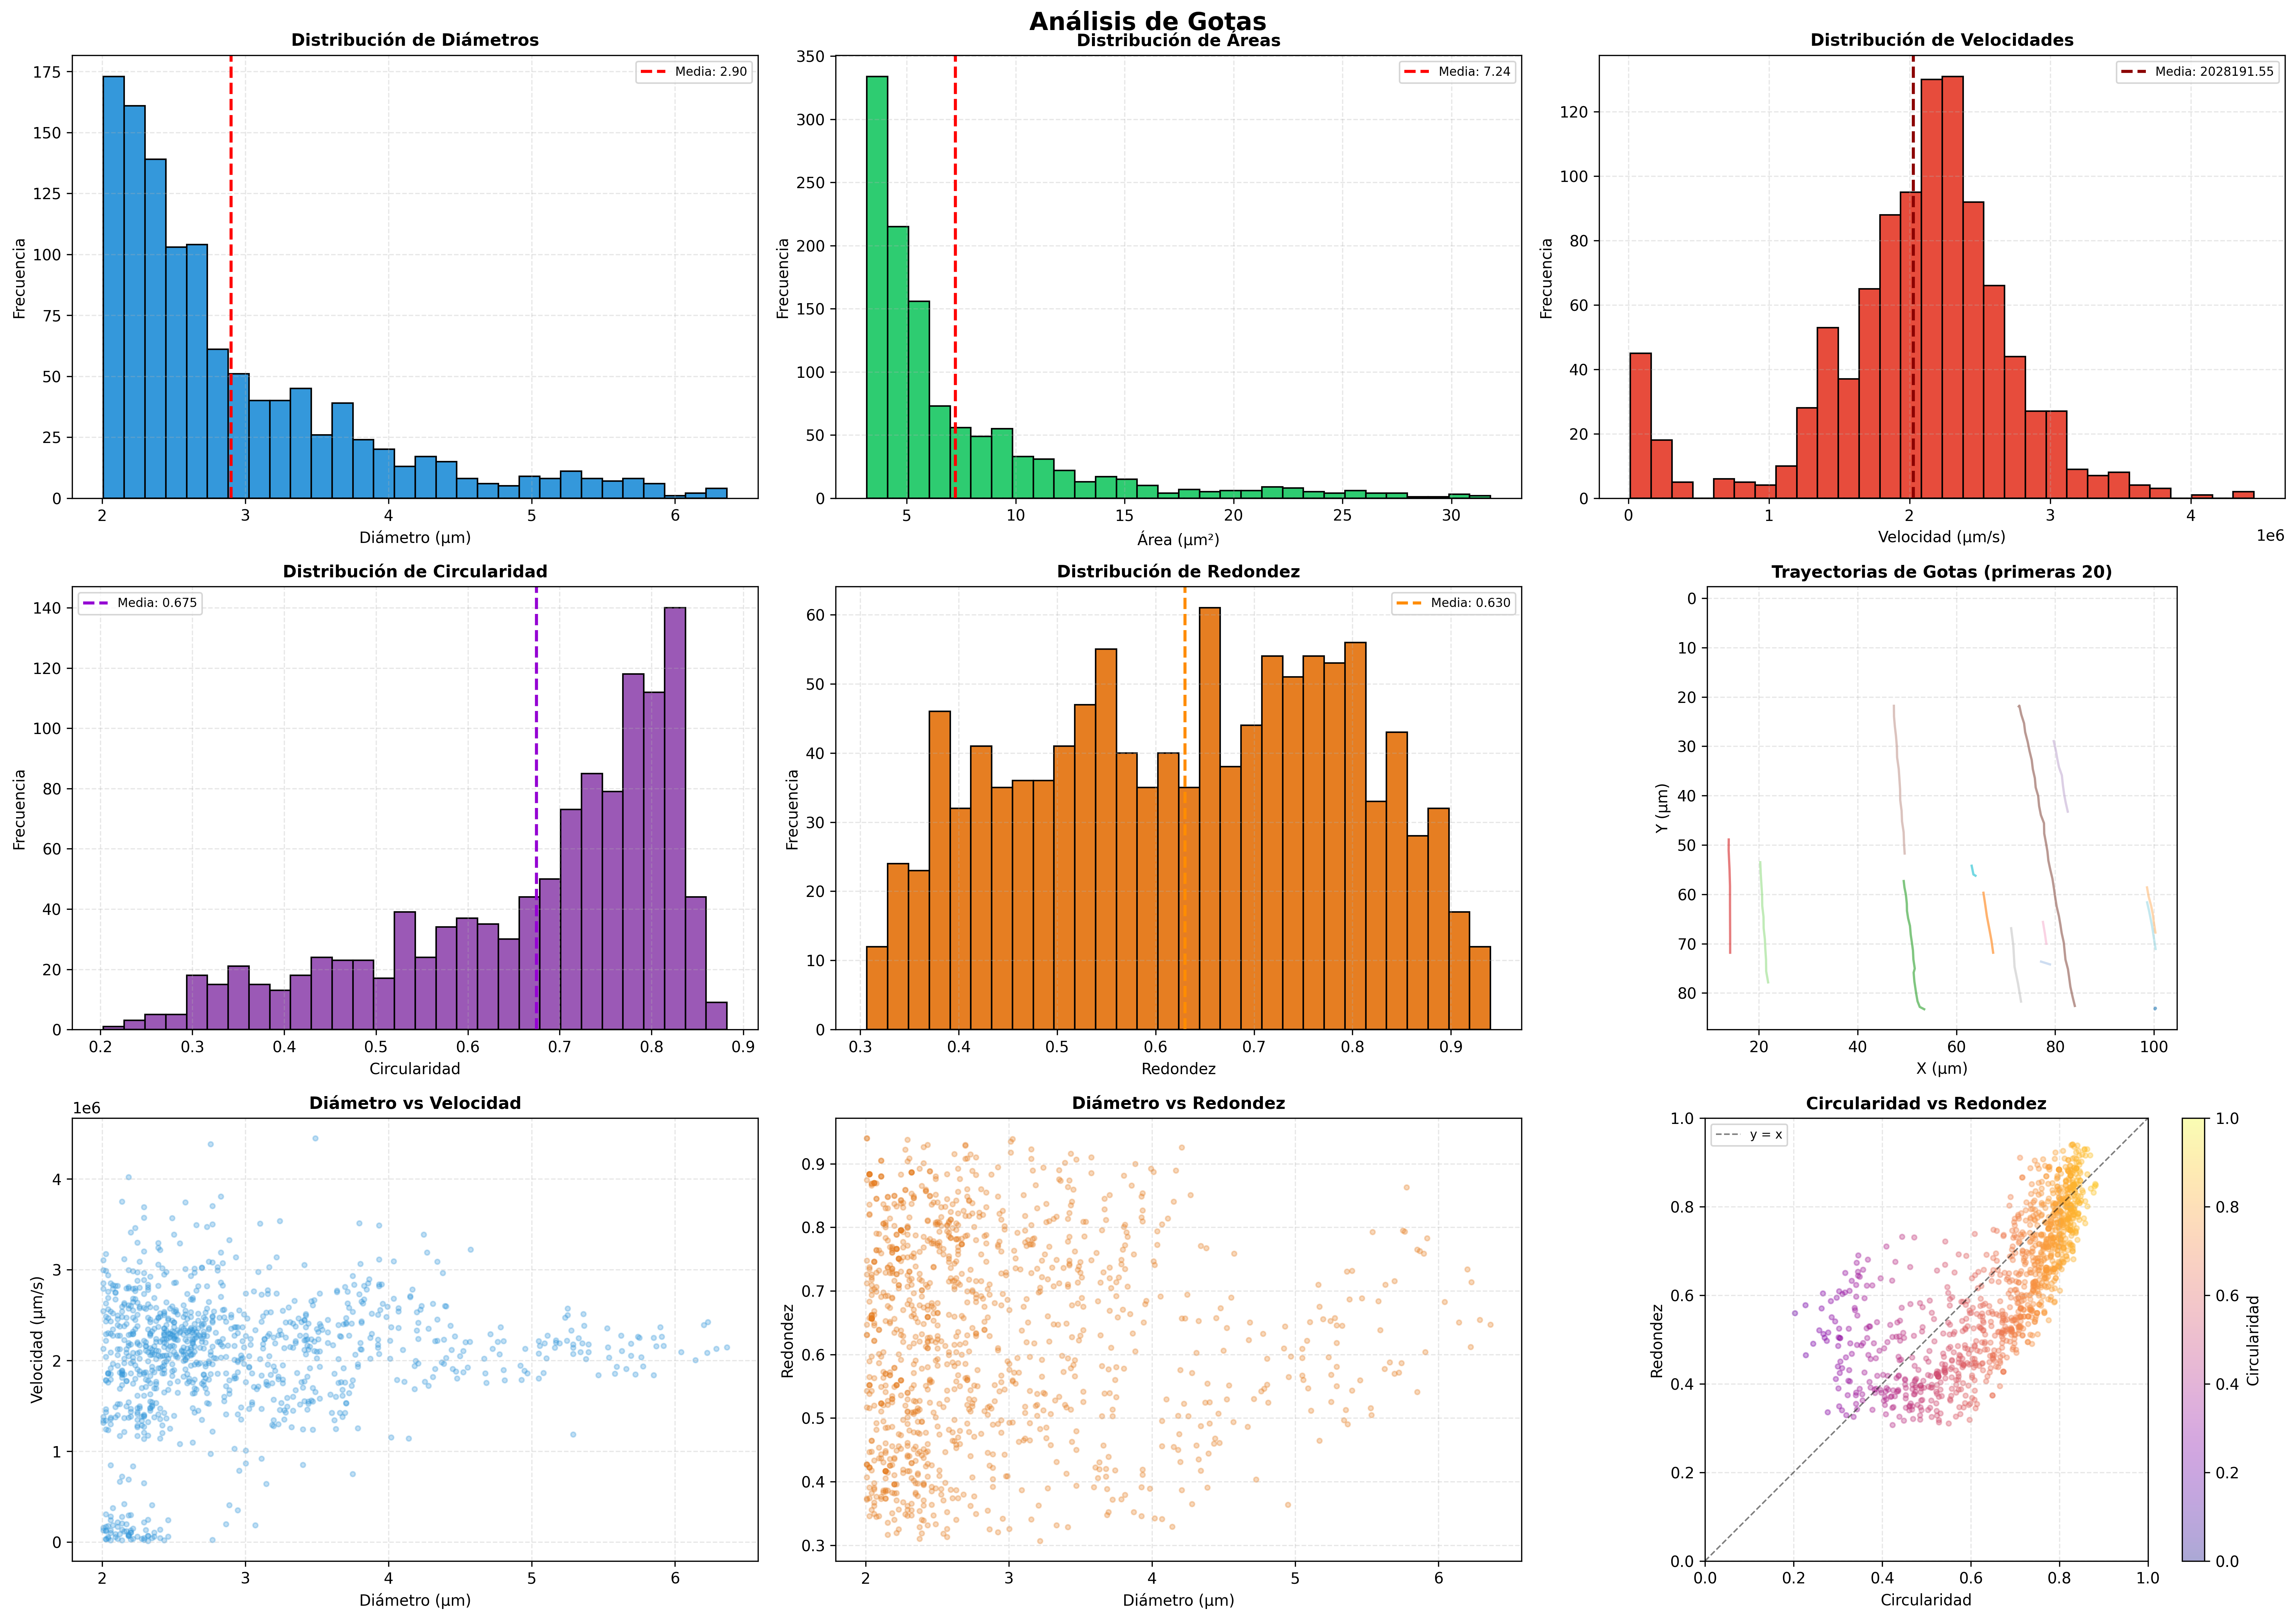
\includegraphics[width=1\textwidth]{figures/manual_usuario/analysis_plots.png}
    \caption{Ejemplo de las gráficas generadas.}
    \label{fig:graficas}
\end{figure}
